%!TEX root = ../../thesis.tex


\section{Double Layers}
  \label{sect:background_doubleLayers}


  Modelling and measuring the electrical aspects of interfacial double layers draws on both electronic and chemical concepts.
  Those with an electronic background are unlikely to be familiar with double layers.
  This section provides background on what a double layer is and how one is formed, beginning with a discussion of liquids.


  \subsection{Formation}
    \label{sub:background_doubleLayers_formation}


    % Water
    \begin{figure}
        \begin{center}
            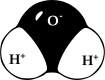
\includegraphics{content/introduction/graphics/polarWater}
        \end{center}
        \caption{Molecular model of the water molecule}
        \label{fig:waterMolecule}
    \end{figure}
    A double layer is an organised layer of liquid; two layers to be precise.
    Because double layers are a property of liquids, and most common liquids are water based, the properties of water is an appropriate place to start.
    The following properties of water are not necessary for the formation of double layers, but knowing of them helps build a mental model of the system.
    At the microscopic scale, individual atoms and molecules within liquids interact with complexity.
    The density of atoms and molecules in water is extreme, $3.33\times10^{22}$ \ce{H2O} molecules per millilitre.
    These molecules are polar, meaning that one side appears negatively charged while the other appears positively charged, shown in~\cref{fig:waterMolecule}.
    This causes them to respond to electric fields by rotating, so as to minimise their potential energy in the field.
    Because of this, any ions present become surrounded by arranged volumes of water.
    For example, a positive ion will be surrounded by water molecules orientated such that their hydrogen atoms all point away from the ion.
    It is also possible for water to spontaneously disassociate from \ce{H2O} into a proton (\ce{H+}) and a hydroxide anion  (\ce{OH-}).

    % Formation
    To form a double layer a liquid containing ions must meet a solid object with charged trapped at its surface.
    Once this happens, the ions within the liquid are drawn to, or repelled from, the solid's surface.
    The point where the two states of matter meet is called the interface.
    Those ions that have been drawn to the interface collect together to form a double layer.
    Double layers occur when using pure water as the liquid, because of its ability to disassociate, but mostly it is the ions from an electrolyte solution that form the layer~\cite{Bruesch2004}.
    The double layer is simply the collection of ions drawn from a liquid to the surface of a solid.


    % Shielding
    \begin{figure}
        \begin{center}
            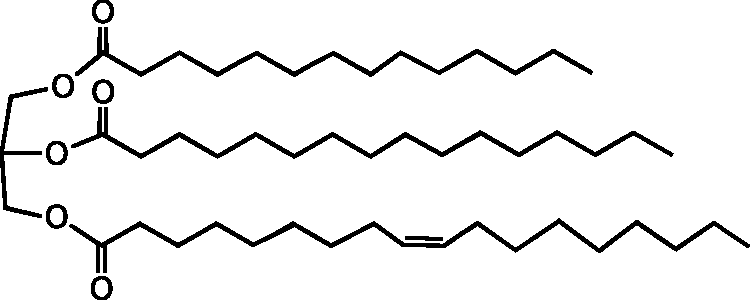
\includegraphics[scale=0.8]{content/introduction/graphics/butterfat}
        \end{center}
        \caption{Structural formula of a butterfat molecule}
        \label{fig:butterfat}
    \end{figure}
    The term `solid' may refer to the walls of a container or particulates suspended in solution.
    When a particulate is suspended throughout a solution it is referred to as an emulsion.
    For example, milk is such an emulsion of butterfat in water.
    \Cref{fig:butterfat} shows the structure of a butterfat molecule; a long structure that behaves as a solid.
    The stability of an emulsion, such as milk, depends on the strength of the double layers that encapsulate each particle.
    These double layers shield the molecules or particles from one another electrically.
    By shielding them from each other they are unable to collect and bond together.
    This shielding prevents milk from coagulating and turning to lumps.

    %% Interfaces
    %\begin{figure}[h]
        %\begin{center}
            %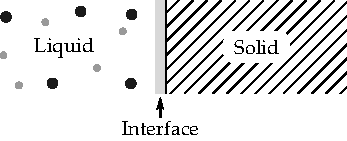
\includegraphics{content/introduction/graphics/simpleLayerDiagram}
        %\end{center}
        %\caption{Diagram showing the location of the fluid-solid interface}
        %\label{fig:interfaceDiagram}
    %\end{figure}
    %The boundary between any two states of matter is referred to as an interface; it is simply where two things meet.
    %We are interested specifically in the dynamics of the solid-liquid interface.

    %Interactions relevant to double layers occur in a thin region inside the liquid at the interface.
    %When there is a difference in charge between the solid surface and the liquid bulk, a double layer forms.
    %The following three statements are capture underlying nature of double layers.
    %\begin{itemize}
      %\item The charged elements in a solid are fixed in place, but in a liquid they are free to move.
      %\item Any charge imbalance between solid and liquid will be greatest at the point they meet.
      %\item Charges interact with each other, whether by repulsion or attraction.
    %\end{itemize}
    %The consequence being that any charge interactions will be most pronounced within the liquid phase at the surface of the solid.


    Having addressed where double layers come from, as well as their organisation, the anatomy of these layers is now introduced.


  \subsection{A physical model}
    \label{sub:background_doubleLayers_physicalModel}


    \begin{figure}
      \begin{center}
        
\includegraphics{content/introduction/graphics/counterAndCoIons}
      \end{center}
      \caption{Counter-ions are oppositely charged, co-ions have like charge.}
      \label{fig:counterAndCoIons}
    \end{figure}
    In the previous section, a brief explanation of what a double layer is and where they form was introduced.
    We next look at double layer anatomy and define some of its properties.
    Before moving on, use of the terms `co-ion' and `counter-ion' is defined.
    These terms refer to ions containing charge -- like or opposite -- in polarity to a second charge or body of charge.
    For example, if a negatively charged surface attracts positively charged ions then positive ions are the counter-ion.
    Likewise, if a positively charged surface was to repel a positive ion then the positive ion is the co-ion.
    The terms are convenient because they remove the need to identify specific polarities during discussion.
    This relationship is shown in~\cref{fig:counterAndCoIons}.

    \begin{figure}
      \begin{center}
        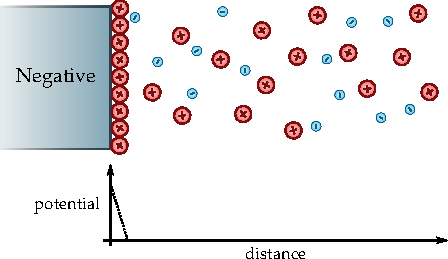
\includegraphics{content/introduction/graphics/model_helmholtz}
      \end{center}
      \caption{Structure of the Helmholtz layer.}
      \label{fig:doubleLayerModel_helmholtz}
    \end{figure}
    Three models of the interfacial double layer have been proposed over time.
    Each represents an extension or modification of the previous, beginning with the Helmholtz Model~\cite{Horch2004}.
    Helmholtz proposed his parallel plate capacitor based model in 1879~\cite{Geddes1997}.
    His model consists of two layers of surface charge, one inside the solid and one in the liquid.
    The counter-ions sit in a \emph{compact layer}, meaning that they are bound to the surface and immobile.~\cite{Salieb-Beugelaar2009}
    Figure \ref{fig:doubleLayerModel_helmholtz} represents this as a row of tightly packed positive ions along the solid surface.
    Past the layer of bound surface ions there is no effect from the charged surface of the solid.
    In essence, his model defines the interface a single layer of ions held against the edge of a solid.
    The problem with this model is its inability to predict the layer's capacitance.
    Measured capacitance of a double layer depends on the potential difference across the layer, and the concentration of ions in the solution~\cite{Bard1980}.
    Helmholtz's model does not account for the dependence of capacitance upon the potential difference and concentration and therefore is not an accurate representation.

    \begin{figure}
      \begin{center}
        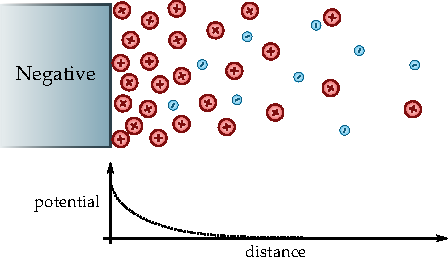
\includegraphics{content/introduction/graphics/model_guoyChapman}
      \end{center}
      \caption{Structure of the Goüy-Chapman layer.}
      \label{fig:doubleLayerModel_gouyChapman}
    \end{figure}
    Later, Goüy and Chapman independently proposed that charge in the liquid phase may instead be held in a \emph{diffuse layer}~\cite{Chapman1913}.
    This meant that ions in the layer were not fixed and that the density of charge in the layer could vary.
    Figure~\ref{fig:doubleLayerModel_gouyChapman} illustrates the concept by the lack of ions bound to the surface and the gradual decline in counter-ion concentration with distance from the surface.
    The Goüy-Chapmam Model accounts for the observed variation in capacitance by distributing charge in the liquid as a gradient from the surface of the solid.
    The layer is free to change its concentration profile in response to applied electrostatic potential and ionic concentration.
    In the case of a higher electrostatic potential, the layer is pulled closer to the surface, becoming shallower.
    In the case of a higher electrolytic concentration, the layer is more concentrated with a higher charge density, again becoming shallower.
    It predicts the change in capacitance by growing or shrinking the size of the layer, but it still fails to predict the capacitance at high ionic concentrations.
    This is in part because it fails to account for the physical size of the ions in the electrolyte and instead models them as point charges~\cite{Bard1980}.
    In their model, ions can get infinitely close to the surface regardless of their size.
    This becomes a problem at high ionic concentration where the surface becomes crowded.

    \begin{figure}
      \begin{center}
        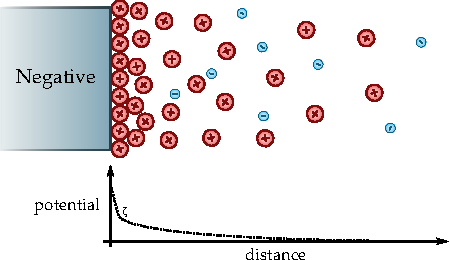
\includegraphics{content/introduction/graphics/model_stern}
      \end{center}
      \caption{Structure of the Goüy-Chapman-Stern layer.}
      \label{fig:doubleLayerModel_stern}
    \end{figure}
    In 1924, Otto Stern published his modified version of the Goüy-Chapmam model~\cite{Stern1924}.
    This model, illustrated in figure~\ref{fig:doubleLayerModel_stern} extends the Goüy-Chapmam model by setting the minimum distance an ion can get to the solid surface.
    This effectively reintroduces the compact layer as seen in Helmholtz's model but allows for a concentration gradient exterior to this layer.
    It resembles the Helmholtz model at high ionic concentration but accounts for spread in the layer dimensions at lower concentrations.
    The Stern, sometimes referred to as the Goüy-Chapmam-Stern, model is a well accepted double layer model~\cite{Olthuis2005}.


  \subsection{Structure/anatomy}
    \label{sub:backgound_doubleLayers_anatomy}


    \begin{figure}
      \begin{center}
        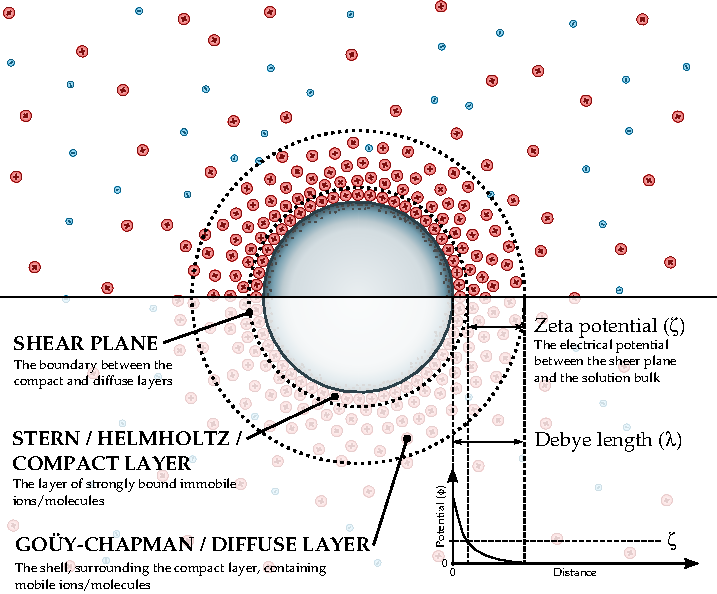
\includegraphics{content/introduction/graphics/doubleLayer_version2}
      \end{center}
      \caption{Anatomy of the double layer}
      \label{fig:doubleLayer_anatomy}
    \end{figure}
    Figure~\ref{fig:doubleLayer_anatomy} shows the double layer organisation according to the currently accepted Goüy-Chapmam-Stern model.
    It shows the compact layer adsorbed to the surface of the suspended solid.
    In this layer the ions are immobile due to the electrical strength at the surface.
    Surrounding this layer is the diffuse layer.
    Ions here are still drawn to the solid, but not so strongly as to be immobile.
    The electric potential in this layer decays from that within the compact layer to the potential in the bulk of the solution.
    These layers are divided by the shear plane.
    The shear plane represents nearest distance from the surface at which the layer can move laterally.
    This is an important parameter with linear geometries, such as the inside of a pipe, as it represents the true no-slip boundary.
    The thickness of a typical double layer is between \SI{1}-\SI{100}{\nano\meter}~\cite{Jiang2010}, as defined by its Debye length~\cite{Israelachvili2011}.
    The Debye length is the distance between the interface and the point in the liquid where the electric potential is no longer affected by the charged interface.
    As mentioned in the previous section, this varies based on the ionic concentration of the solution and the potential at the solid surface.


  % Marcus Wilson tore this apart, don't even mention computer simulation.
  %\subsection{Liquid simulation}
    %\label{sub:molecularSimulation}


    %At the macroscopic scale, liquid behaviour is simple and calculable.
    %Modern computers can simulate the movement of liquids using the Navier-Stokes equations with accuracy and speed.
    %Engineers simulate the flow of liquids, or any Newtonian fluid, routinely using computer design tools.
    %These tools allow engineers to push boundaries of aircraft and boat design.
    %However, this does not hold true when modelling fluid at the microscopic scale due to the required scale.
    %%Computer simulations are  based upon calculating the state of a system of objects at specific time intervals.
    %%There are other methods, such as
    %%At each computed time interval the variables of each element of a system are updated and the cycle repeats.
    %%This repeats for every time-step until the simulation time-frame has run its course.
    %%These simulations are not run in real-time; instead taking hours or days to compute simulations spanning fractions of a second.

%%    Finite-difference time-domain simulation is a common technique for calculating electrical fields and resulting currents and voltages in the field of electrical engineering.
%%    Such simulations can involve hundreds of thousands, \emph{sometimes millions}, of objects.
%%    These objects are elements of a 3D mesh created to represent the geometry of the system.
%%    Because of the dependence on neighbouring parameter values, each time-step may take many passes over each element in a system to calculate the final state before moving on.
%%    This type of simulation is common whenever the effects of radio waves need to be simulated.

    %Designing and conditioning computer simulations at a molecular scale are challenging.
    %Simulating the interface is possible, but is very involved and constitutes a field of its own.
    %The work of Nagy et al.\ ~\cite{Nagy1992} and Bazant et al.\ ~\cite{Bazant2011} has shed light on some of the underlying physical mechanics of the double layer.
    %Matters are complicated by the fact that some aspects of the double layer are still not fully understood~\cite{Kornyshev2007}.

    %Simulation of a liquid having a sensible macroscopic volume is impractical.
    %The molar mass of water is \SI{18.0528}{\gram\per\mole}.
    %One gram of water is defined as one millilitre, so we can say that for every millilitre of water we have we have an eighteenth of a mole of water.
    %Avagadro's constant, the number of constituent particles per mole of a given substance, is $6.0221\thinspace \times 10^{23}$.
    %Therefore we have one eighteenth of Avagadro's constant in water molecules, which is about $3.3333\times 10^{22}$ molecules.
    %Molecular simulation has not been employed here.
    %Useful results are likely to be obtained from volumes less than \SI{1}{\milli\litre}, but the time and resources to successfully run and validate such simulations are high.
    %Such simulations are shaping the underlying models of the interfacial double layer~\cite{Kornyshev2007}.


\section{Streaming Cells}
  \label{sect:background_streamingCells}


  % Double layes on flat surfaces
  \begin{figure}
      \centering
      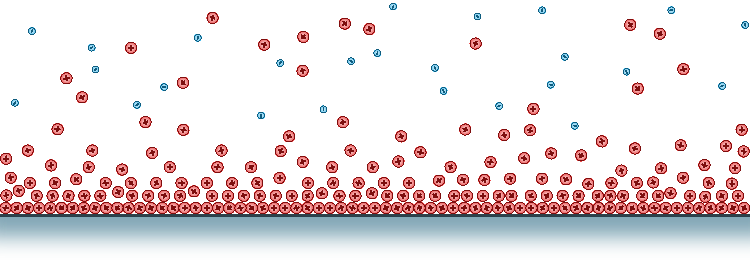
\includegraphics{content/pt1/01-PowerHarvesting/graphics/intro_2_wall}
      \caption{
        \label{fig:doubleLayerBetweenWalls}
        Formation of a double layer along a solid wall.
      }
  \end{figure}
  Consider a double layer that has formed along a perfectly flat surface.
  \Cref{fig:doubleLayerBetweenWalls} illustrates this situation, where the walls are negatively charged and therefore the counter-ions are positively charged.
  Counter-ions, separated from the bulk of the liquid, line the exterior of the wall; but charge separation is not enough to generate electrical power.

  % Harvesting energy
  \begin{figure}
      \centering
      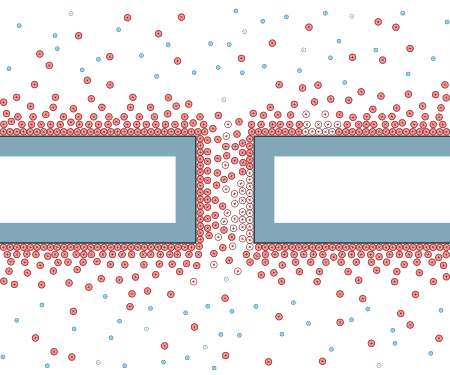
\includegraphics{content/pt1/01-PowerHarvesting/graphics/intro_2_channel_relaxed}
      \caption{
        \label{fig:doubleLayerInChannel_noPressure}
        Double layer formation within a streaming cell that is in a state of equilibrium.
      }
  \end{figure}
  Energy can not be created or destroyed, it must be converted from one form to another.
  In this case, counter-ions are electrostatically bound to the interface and removing them requires work.
  Although the counter-ion density has been increased at the boundary, the charge is not free.
  Migration of charge to the walls ceases once the surface potential has been neutralised.
  Double layer formation takes work to undo and the process stops once the layer is formed.
  Generating electrical energy requires taking some form of power from the fluid, in this case mechanical.
  Liquids pass mechanical power in the form combination a pressure and a flow.
  Harvesting power from liquid will cause a drop in pressure as liquid is pushed through the harvesting mechanism.
  The mechanisms presented here use mechanical power to shift the ionic balance between two bodies of liquid.
  This means separating and isolating negative and positive ions from each other.
  Figure~\ref{fig:doubleLayerInChannel_noPressure} shows another charged wall, but with the addition of a small channel.
  Notice that the channel contains no co-ions, it is exclusively occupied by counter-ions.
  The ratio of counter-ions to co-ions within the channel is controlled by the width of the channel.
  The narrower the channel, the less likely it is for co-ions to get inside.
  This channel is small enough that the layers overlap one another, repelling co-ions.
  The channel and the two separated bodies of liquid now form an energy harvester.
  Counter-ion rich fluid is transported across the channel by applying a pressure differential.
  As counter-ions exit the channel on the low-pressure side, new ions move to replenish the double layer on the high-pressure side.
  \begin{figure}
      \centering
      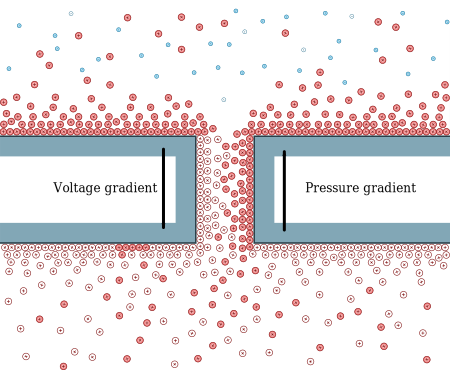
\includegraphics{content/pt1/01-PowerHarvesting/graphics/intro_2_channel}
      \caption{\label{fig:doubleLayerInChannel_withPressure}Double layer formation within a streaming cell that has a pressure differential applied.}
  \end{figure}
  A diagram showing the channel geometry, but with pressure applied and a voltage gradient generated is shown as figure~\ref{fig:doubleLayerInChannel_withPressure}.
  The two walls and channel is referred to as a streaming cell.
  Streaming cells are able to continuously separate ions of an electrolyte fluid.
  Electrical potential across a streaming cell increases as those ions are pumped through.
  This only works when the solid surface has charge at its surface, necessary to form the double layer.

  % Channel fabrication and materials
  A channel can be created individually using a range of fabrication methods, such as chemical etching or using narrowly separated parallel plates.
  They can also be formed en masse by using porous materials such as glass or ceramics, where the pores themselves act as channels.
  Glass has the convenient property that it spontaneously obtains a negative surface charge when in contact with water, the requirement for double layer formation.
  This surface charge is caused by the deprotonation of surface silanol groups in glass (SiOH~$\leftrightarrows$~SiO$^{-}+$~H$^{+}$)~\cite{Kirby2004}.
  By immersing a glass channel in an electrolyte solution, the glass donates protons into the solution leaving its surface negatively charged.
  In turn, positively charged double layers line the channel's inner walls ready to be pumped through the channel.
  This means that glass channels have a higher voltage on the low-pressure side and a lower voltage on the high-pressure side.

  % Limitations of previous content
  The concept behind the device is relatively straight-forward, but the physical reality is complex.
  The diagrams presented here are simplified, having perfectly flat walls containing single atom ions carrying a single charge.
  No mention of molecules has been made, which increases the complexity.
  Polar molecules such as water have positive and negative components offset in space.
  Although simplified, this material illustrates the how streaming cells work.
  Next, literature concerning the operation, design and improvements to streaming cell technology is presented and discussed.


  \subsection{Literature review}
    \label{sub:background_streamingCells_literatureReview}


    % Initial work of Osterle
    \begin{figure}
      \centering
      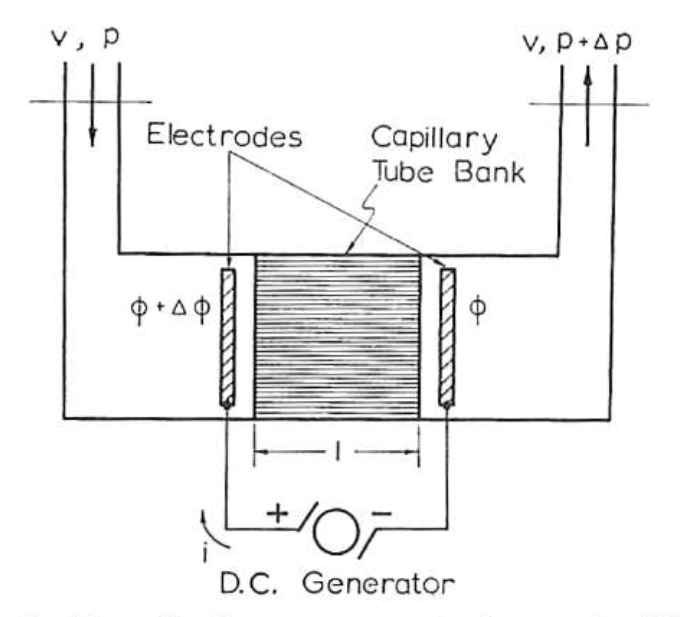
\includegraphics[height=6cm]{content/pt1/Osterle_ElectrokineticCell.png}
      \caption{\label{fig:Osterle_cell}Osterle's electrokinetic pumping cell, reproduced from \cite{Osterle1964}}
    \end{figure}
    In 1964, a paper by Osterle gave an analysis of energy conversion from streaming cells, both for the purpose of pumping fluid or generating electrical power was presented~\cite{Osterle1964}.
    The cell he used consisted of fine capillary tubes stacked together to form a streaming cell.
    A diagram of that cell, in its pumping configuration, is reproduced here as~\cref{fig:Osterle_cell}.
    Importantly, he shows that a streaming cell has the same conversion efficiency whether it is in a pumping mode, where electrical energy is supplied, or in a generating mode, where electrical energy is produced.
    Based on his analysis, Osterle gives an illustrative example of a streaming cell producing electrical energy.
    He states that tube bank having a volume of \SI{100}{\centi\meter\cubed} with \SI{100}{\kilo\pascal} of hydrostatic pressure applied would be capable of producing \SI{0.49}{\watt} of electrical energy.
    This would require \SI{125}{\watt} of pumping power to achieve, giving an energy conversion efficiency of \SI{0.392}{\percent}.

    % Another, paper - the beginning of streaming cells
    Within the space of a year three papers related to properties of fluid flow in fine capillaries, such as those used by Osterle are presented.
    Burgreen and Nakache investigate both the flow when the capillaries are rectangular~\cite{Burgreen1964}, and the efficiency of such capillaries when used to generate electrical power or to pump~\cite{Burgreen1965}.
    Their work develops mathematics behind rectangular streaming cells and shows fine glass capiliaries are equally efficient when used to generate electrical power or to induce liquid pumping.
    Rice and Witehead make an analysis of fluid flow profiles that consider the effect of double layer interactions~\cite{Rice1965}.
    They show how the double layer affects the level to which liquid can permeate a material populated with cavites.
    Together these three papers mark the beginning of research into streaming cells.

    % Renewed interest and dimensions
    There appears to be little published research into streaming cells until 2003, when a surge of papers related to optimal dimensions of streaming cells appear.
    An analysis relating energy conversion efficiency to the length of a streaming cell channel indicated that short cells are the most efficient~\cite{Yang2003}.
    However, more recent work by Chang and Yang shows a decrease in conversion efficiency at maximum power when the channel length is low~\cite{Chang2009}.
    This work suggests there is an optimum channel length, which is also dependent on the fluid conductivity.
    Investigation into the relationship between the Debye length of the double layer and streaming cell conversion efficiency found that a channel is most efficient when its height is twice that of the Debye length~\cite{Daiguji2004}
    This corresponds to the point at which double layers formed within a cell begin to overlap with one another.

    In 2005 a seminal paper by van der Heyden et al.\ reported on streaming cell measurements made in a single micro-channel \SI{70}{\micro\meter} in height~\cite{VanderHeyden2005}.
    Many valuable contributions were detailed in this paper, namely:
    \begin{enumerate}
      \item Confirmed that reversing the polarity of surface potential reverses the direction of the streaming current.
      \item Found that the maximum conversion efficiency corresponded to channels where double layers begin to overlap. This confirms the relationship put forward the previous year by Daiguji et al.\
      \item Showed that boundary conditions involving constant surface potentials, used up to this point to model streaming, are inaccurate.
      \item Predicted a maximum energy conversion efficiency of $\sim$\SI{6}{\percent} for potassium chloride solutions of \SI{1e-5}{\mole} in silica channels of height \SI{145}{\nano\meter}.
    \end{enumerate}
    Subsequent research by the same authors show that conversion efficiency is maximised at low salt concentrations~\cite{VanderHeyden2006}.
    They also predict an energy conversion efficiency of \SI{12}{\percent} for streaming cells using electrolyte solutions containing lithium.
    Around the same time, Daiguji et al.\ publish work suggesting that in order to increase cell efficiency one may either reduce the channel height or decrease the ionic concentration of the working fluid~\cite{Daiguji2006}.
    This supports the work of van der Heyden et al.\ with respect to efficiency gains with the working fluids having low ionic concentrations.

    % Stern conductance
    In 2007, van der Heyden et al.\ publish a measured energy conversion of \SI{3.2}{\percent}~\cite{Heyden2007}.
    They suggest that the conversion efficiency of a channel is limited by a property termed `Stern conductance'.
    The concept of Stern conductance is that the Stern layer (see \cref{fig:doubleLayer_anatomy}) itself provides a pathway for electrical conduction.
    This conduction turns the surface of the glass into an electrically conductive surface causing the cell to partially self-discharge.
    Stern conductance is often referred simply as `surface conductance'.
    Davidson and Xuan published a mathematical model shortly after confirming the role of Stern conductance on streaming cells, in particular those with low ionic strength~\cite{Davidson2008}.
    They suggest that this is the reason for poor measured efficiencies in light of the much higher predicted values.

    % Hydrodynamic slip
    \begin{figure}
      \centering
      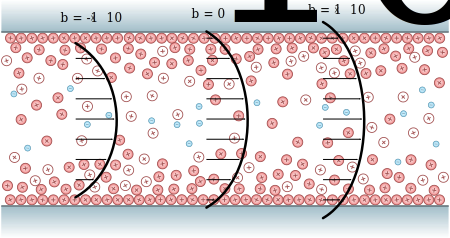
\includegraphics[height=6cm]{content/pt1/graphics/HydrodynamicSlip}
      \caption{\label{fig:HydrodynamicSlip}Illustration of hydrodynamic slip inside a channel cavity, where $b$ is the slip length. Arrows indicate flow velocity in each of the three situations.}
    \end{figure}
    Most recently, the concept of hydrodynamic slip has been applied to streaming cells as a way of increasing conversion efficiency.
    Estimates using mathematical models predicted conversion efficiencies between \SI{30}{\percent} and \SI{70}{\percent}~\cite{Pennathur2007, Davidson2008a, Ren2008}.
    Hydrodynamic slip refers to the ability of a fluid to `slip' relative to a boundary/interface.
    Slip is advantageous to streaming cells because it permits ions in the Stern layer to move relative to the wall.
    The length refers to an imaginary distance into the solid wall where the traditional `no-slip' boundary condition would occur (refer to~\cref{fig:HydrodynamicSlip}).
    A `no-slip' boundary condition dictates that fluid at the boundary of a solid must have zero velocity.
    This condition, along with viscosity, is responsible for the parabolic flow profile a fluid takes as it moves through pipes.
    An issue surrounding slip was illustrated by Eijkel who showed that a channel's zeta potential and its slip length are linked~\cite{Eijkel2007}.
    The general problem with slip-based mechanisms is that a high zeta potential is optimal for double layer formation, however it also promotes wetting.
    Wetting and hydrodynamic slip are related to each other by the strength of attraction between a liquid and a solid.
    To explain, the terms hydrophobic and hydrophilic are used to describe surfaces that repel and attract water.
    A hydrophobic surface has a low tendency to support water, i.e., water will bead and roll off a hydrophobic surface.
    Conversely, a hydrophilic surface is one that water \emph{is} attracted to, causing a droplet to spread and stick to the surface.
    Hydrodynamic slip occurs when a channel's walls are hydrophobic, allowing water at the interface to slip along the boundary of the solid.
    High zeta potentials attract water to the solids surface due to electrostatic attraction.
    Eijkel's publication illustrates that the zeta potential and hydrodynamic slip are related to one another.
    In order to improve the situation in steaming cells a surface should be both non-wetting and hold a high surface charge.
    Conservative estimates place an efficiency of \SI{40}{\percent} on cells having slip lengths tens of nanometres long, obtainable using carbon nanotubes, using solutions having low salt concentration.


    %Research around streaming cell energy conversion headed in a new direction after an article written by Pennathur et al.\ in 2007 detailed a mathematical model predicting the effects of hydrodynamic slip~\cite{Pennathur2007}.
    %It proposed efficiency figures as high as \SI{30}{\percent} for a slip length of \SI{6.5}{\nano\meter} in cylindrical tubes \SI{100}{\nano\meter} in diameter.


    %Eijkel, in a follow-up publication to that of Pennathur's, discusses the relationship between zeta potential and slip length~\cite{Eijkel2007}.

    %\begin{figure}
      %\centering
      %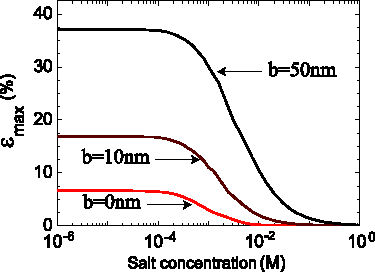
\includegraphics[height=6cm]{content/pt1/graphics/SteinSlipEnchancedChannelEfficiency}
      %\caption{\label{fig:Stein_Slip_Prediction}Plot of predicted efficiency versus salt concentration for various for slip lengths of 0, 10 and \SI{50}{\nano\meter}, taken from~\cite{Ren2008}.}
    %\end{figure}

    %That same year, two papers modelling the effects of hydrodynamic slippage were published.
    %The first, by Davidson and Xuan, gives a mathematical prediction of the effects of hydrodynamic slippage at the interface surface~\cite{Davidson2008a}.
    %They predict that when taking slip at the solid-fluid boundary into consideration that conversion efficiencies as high as \SI{30}{\percent} should be obtainable.

    %The second, by Ren and Stein, predict conversion efficiencies as high as \SI{70}{\percent} based on the slip lengths recently observed with carbon nanotubes~\cite{Ren2008}.
    %They provide a more conservative prediction of \SI{40}{\percent} for slip lengths in the tens of nanometers region and low salt concentration.

    % Summary
    Theoretical predictions of the efficiency of standard micro/nano-fluidic channels are 2\% for pure water and 7\% for sodium chloride.~\cite{VanderHeyden2006}
    However, measured conversion efficiencies as reported thus far are:
    \begin{itemize}
      \item ``far less than \SI{1}{\percent}'' forcing potassium chloride through a porous glass plug having pores in the range \SI{1}--\SI{1.6}{\micro\meter}~\cite{Olthuis2005}.
      \item 0.01\% by forcing water through porous glass with pore sizes from 10\thinspace--\SI{16}{\micro\metre}.~\cite{Yang2003}
      \item 0.8\% by forcing pure water through a ceramic rod populated with \SI{6}{\micro\metre} pores.~\cite{Yang2004}
      \item 3\% by forcing a sodium chloride solution through a \SI{75}{\nano\metre} by \SI{50}{\micro\metre} silica channel.~\cite{Heyden2007}
      \item 0.77\% by forcing a sodium chloride solution through a \SI{200}{\nano\metre} pore in an alumina membrane.~\cite{Lu2006}
      \item 5\% by forcing a sodium chloride solution through a \SI{0.5}{\nano\metre} cylindrical pore in polyethylene terephalate foil.~\cite{Xie2008}
    \end{itemize}
    It is clear from the literature that there is significant progress to be made with respect to increasing the conversion efficiency of streaming cells.
    Techniques to induce hydrodynamic slip at the fluid-solid interface are predicted to increase this efficiency to 30-40\%~\cite{Davidson2008a, Ren2008}, but progress in this area is dictated by advancements in materials science.
    Experimental results utilising slip enhanced channels have not yet been reported in the literature.
    Surface enhanced channels will not be investigated due to manufacturing difficulty, cost, and the level of scientific development required to make progress.

    %In 2012, Cherng Hon et al.\ presented a novel method of producing electrokinetic power from steaming cells using salinity gradients~\cite{CherngHon2012}.
    %In this work the authors describe a system where flow through a conventional streaming cell is brought about by forward osmosis.
    %This allows the authors to generate electrical energy from streaming cells without mechanical pumping.
    %The application has limited use, but it highlights novel uses for streaming cells as a means of electrical generation.

    %Most recently, in 2014, Jiao et al.\ presented results showing that surface treatment of porous glass can increase conversion efficiency~\cite{Jiao2014}.
    %They show that ultrasonically pre-treating glass and subsequently applying Sodium Dodecyl Sulphate to the surface gave a relative increase of \SI{27.3}{\percent} in power density.
    %Unfortunately, they do not state the absolute efficiency of their channels in either case.

    %Theoretical predictions of the efficiency of standard micro/nano-fluidic channels are 2\% for pure water and 7\% for sodium chloride.~\cite{VanderHeyden2006}
    %Experimental results show conversion efficiencies in the range of:
    %These results indicate that small channels using solutions containing salt are more efficient.
    %According to \cite{Daiguji2004}, the efficiency is maximised when the channel height is twice that of the Debye length.
    %Additionally, ~\cite{VanderHeyden2006} states that the maximum efficiency is found when the salt concentration is low.

    In summary, the finding that maximum conversion efficiency occurs at low ionic concentration supports the use of tap-water as a working fluid.
    Using glass as a substrate seems to be a suitable choice, which is both cost effective and easy to source.
    The dimensions of channels found in the literature suggest that fabricating trial cells is feasible with the equipment available.
    A conversion efficiency of \SI{0.01}{\percent} should be achievable using a porous glass plug.
    This efficiency will be used a baseline to compare measured efficiency from fabricated cells.



\section{Impedance Modelling}
  \label{sect:background_impedanceModelling}

  \begin{figure}
    \begin{center}
      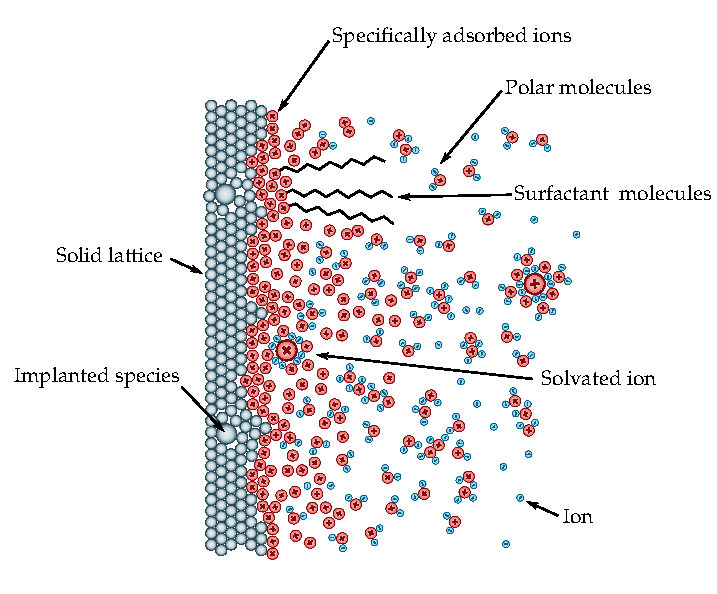
\includegraphics{content/introduction/graphics/interface}
    \end{center}
    \caption{Diagram of an liquid-solid interface showing various types of molecule configurations, surface imperfections and polar molecules. This diagram is based on the work of Bard et al. \cite{Bard1993}}
    \label{fig:interface}
  \end{figure}

  Electronic components have well defined electrical impedances.
  This provides a way to calculate the voltage over a component as a function of time by knowing the current through it, or vice versa.
  For linear devices, such as capacitors, inductors and resistors, this is a relatively simple matter of knowing the size of the device.
  For non-linear devices, such as diodes and transistors, there are models that describe the impedance relationship, which are based on the properties of the materials they are made from.
  But what does an electronic engineer do when there is an electrode-electrolyte-electrode system in their circuit?
  There is no standard model for this situation and trying to calculate the impedance is not trivial.

  Circuit simulators rely on knowing the impedance of components in order to calculate the currents and voltages in circuit branches.
  SPICE is a commonly used circuit simulator that has models of transistors and diodes built in.
  It can easily simulate complex circuits quickly and is a valuable tool for circuit designers as a means of testing their designs before construction.
  However, if the software does not have a model of a component, and the user is not able to describe it, then a circuit simulator is of little use.
  \Cref{part:doubleLayersOnConductors} of this thesis uses a model of an electrode/electrolyte interface to solve some of these problems.
  That interface model can be entered into circuit simulators because it is built of from standard components.
  This means that an electronic engineer can enter it into their design and know what sort of electrical loading to expect between a of electrodes in an electrolyte bath.
  % This allows for the creation of circuit simulation tools, such as SPICE, that predict how a circuit will behave based on its description.
  % Some electronic situations are not so well defined, meaning they can not be entered into circuit simulators.
  % One such situation is when electrodes are inserted into an electrolyte.
  % This would require the simulator to calculate the impedance through the electrolyte, but how do you calculate the impedance of an electrolyte bath?

  In \cref{sect:background_doubleLayers}, illustrations of double layers were presented showing that the interface is comprised of layers.
  A more realistic illustration of a solid-liquid layer is shown in \cref{fig:interface}.
  It shows interactions between polar molecules, between polar molecules and ions, surfactants at the interface, an imperfect solid/liquid boundary, and the the Stern layer.
  The complexity of interactions that happen at the interface are what make is so difficult to model.
  Additional to the interface's impedance is the geometry of the electrodes and the properties of the electrolyte.
  These factors make calculating the impedance between electrodes of an electrode-electrolyte system complex.


  \begin{figure}
    \begin{center}
      \includegraphics{content/introduction/graphics/StJudeOctrode}
    \end{center}
    \caption{Drawing of an eight electrode array used for spinal stimulation. The electrode is called an Octrode and is made by St. Jude Medical.}
    \label{fig:octrode}
  \end{figure}

  To the designers of medical implant devices, estimating the impedance of electrodes in an electrolyte is critical for safe stimulator design.
  Saluda Medical is a recently started company based in Sydney, Australia, developing implantable spinal stimulators.
  Their engineers have designed a stimulator fit for human implantation, but are unsure of the electrical impedance that their implant will see once implanted.
  Getting it wrong could mean their microchip may `latch up'.
  This occurs when one or more pins on a chip goes higher than the supply voltage.
  When this happens, those pins that went above the supply voltage will get stuck on and the only way to turn them off again is to power down the entire chip.
  In an implanted setting this is potentially lethal.
  Naturally, Saluda want a way to model the impedance of electrodes implanted into a human spinal cavity.
  This involves modelling the electrode/electrolyte interface itself, a central idea in interface science.
  \Cref{part:doubleLayersOnConductors} of this thesis looks at ways of doing that using a model of the interface itelf.
  Such a model is suitable for entry into common circuit simulators, such as SPICE, that electronic engineers already use.

